%%%%%%%%%%%%%%%%%%%%%%%%%%%%%%%%%%%%%%%%%%%%%%%%%%%%%%%%%%%%
%% AUFGABE 2
%%%%%%%%%%%%%%%%%%%%%%%%%%%%%%%%%%%%%%%%%%%%%%%%%%%%%%%%%%%%

\newpage
\section{Reaktionsspiel}

In dieser Aufgabe ist ein Reaktionsspiel bestehend aus 5 LEDs und einem Taster zu realisieren. Die LEDs werden nacheinander als Lauflicht ein- und ausgeschaltet. Leuchtet die mittlere LED auf, so muss der Taster gedrückt werden. Reagiert der Spieler rechtzeitig und drückt den Taster während die LED grün leuchtet, so hat er das Level erfolgreich beendet und steigt zum nächsten Level auf. Im nächsten Level läuft das Lauflicht schneller. 

\subsection{Vorbereitung}
\subsubsection{Widerstandsberechnung}

Berechnet:
\[
    R_{V,\text{calc}} = \frac{\SI{5}{\volt} - \SI{2}{\volt}}{\SI{15}{\milli\ampere}} = \SI{200}{\ohm}
\]
Aus E6-Reihe gewählt:
\[
    R_{V} = \SI{220}{\ohm}
\]

\subsubsection{Fragen}

\begin{block}
    \begin{itemize}
    \item[\faQuestion] Wie kann das Mikrocontroller-Programm zu einem beliebigen Zeitpunkt gestoppt werden? Wie kann ausgewertet werden, ob der Taster zum richtigen oder zum falschen Zeitpunkt gedruckt wurde? 
    \end{itemize}
\end{block}

Das Programm kann mittels eines \textbf{externen Interrupts} zu einem beliebigen Zeitpunkt unterbrochen werden. Ein Interrupt wird dazu an einen Pin konfiguriert. 

Sobald der Interrupt ausgelöst wird, springt das Programm direkt in die \textbf{Interrupt-Service-Routine (ISR)}. Dort werden Variablen gesetzt, welche die \texttt{loop}-Methode anschließend überprüft, um den Ablauf zu stoppen. 

Zudem kann in der ISR der aktuelle Status (z.B. welche LED gerade aktiv ist) gespeichert werden. Da der Interrupt sofort reagiert, lässt sich so exakt auswerten, ob der Taster zum richtigen Zeitpunkt gedrückt wurde.


\subsection{Durchführung}

\begin{figure}[h]
\centering
\begin{circuitikz}[scale=0.9, transform shape]

    \draw (0,0) node[above] {D2}
        to[push button, o-, l=$SW_1$] ++ (0,-2)
        to[R, l=$R_1$] ++(0,-2) node[ground]{};
    \draw (2, 0) node[above] {D3}
        to[stroke led, o-, l=$D_1$] ++ (0,-2)
        to[R, l=$R_2$] ++(0,-2) node[ground]{};
    \draw (4, 0) node[above] {D4}
        to[stroke led, o-, l=$D_2$] ++ (0,-2)
        to[R, l=$R_2$] ++(0,-2) node[ground]{};
    \draw (6, 0) node[above] {D5}
        to[stroke led, o-, l=$D_3$] ++ (0,-2)
        to[R, l=$R_2$] ++(0,-2) node[ground]{};
    \draw (8, 0) node[above] {D6}
        to[stroke led, o-, l=$D_2$] ++ (0,-2)
        to[R, l=$R_2$] ++(0,-2)node[ground]{};
    \draw (10, 0) node[above] {D7}
        to[stroke led, o-, l=$D_1$] ++ (0,-2)
        to[R, l=$R_2$] ++(0,-2) node[ground]{};

\end{circuitikz}
\caption{Schaltplan}
\end{figure}

Die für die Durchführung benötigten Bauteile sind in \autoref{tab:bom2} aufgeführt.

\begin{table}[h]
    \centering
    \caption{Stückliste}\label{tab:bom2}
    \begin{tabularx}{\textwidth}{lXXr}
        \toprule
        \textbf{Bez.} & \textbf{Bauteil} & \textbf{Wert} & \textbf{Stückzahl} \\ \midrule
        $R_1$ & Widerstand & \SI{10}{\kilo\ohm} & 1 \\ 
        $R_2$ & Widerstand & \SI{220}{\ohm} & 5 \\ 
        $D_1$ & LED & Red & 2 \\ 
        $D_2$ & LED & Yellow & 2 \\ 
        $D_3$ & LED & Green & 1 \\ 
        $SW_1$ & Taster & & 1 \\ \bottomrule
    \end{tabularx}
\end{table}

\subsubsection{Aufbau am Steckbrett}

Vor dem Aufbau wurde eine Prototyp-Schaltung in Tinker-CAD\footnote{\href{https://www.tinkercad.com/things/4kQIa2P7zRc-2-reaktionsspiel?sharecode=tN5XWwIVhA9dR5oYUQt6OY9f_J_8c10GSfd3RA9Iedc}{Tinker CAD Share Link}} aufgebaut und emuliert, um die Durchführung am Steckbrett zu erleichtern.

\begin{figure}[h]
    \centering
    
\includegraphics[width=.7\textwidth]{tinkercad2.png}
    \caption{Planung des Aufbaus in TinkerCAD.}
\end{figure}

Im Anschluss wurde die Schaltung am Steckbrett aufgebaut.

\begin{figure}[h]
    \centering
    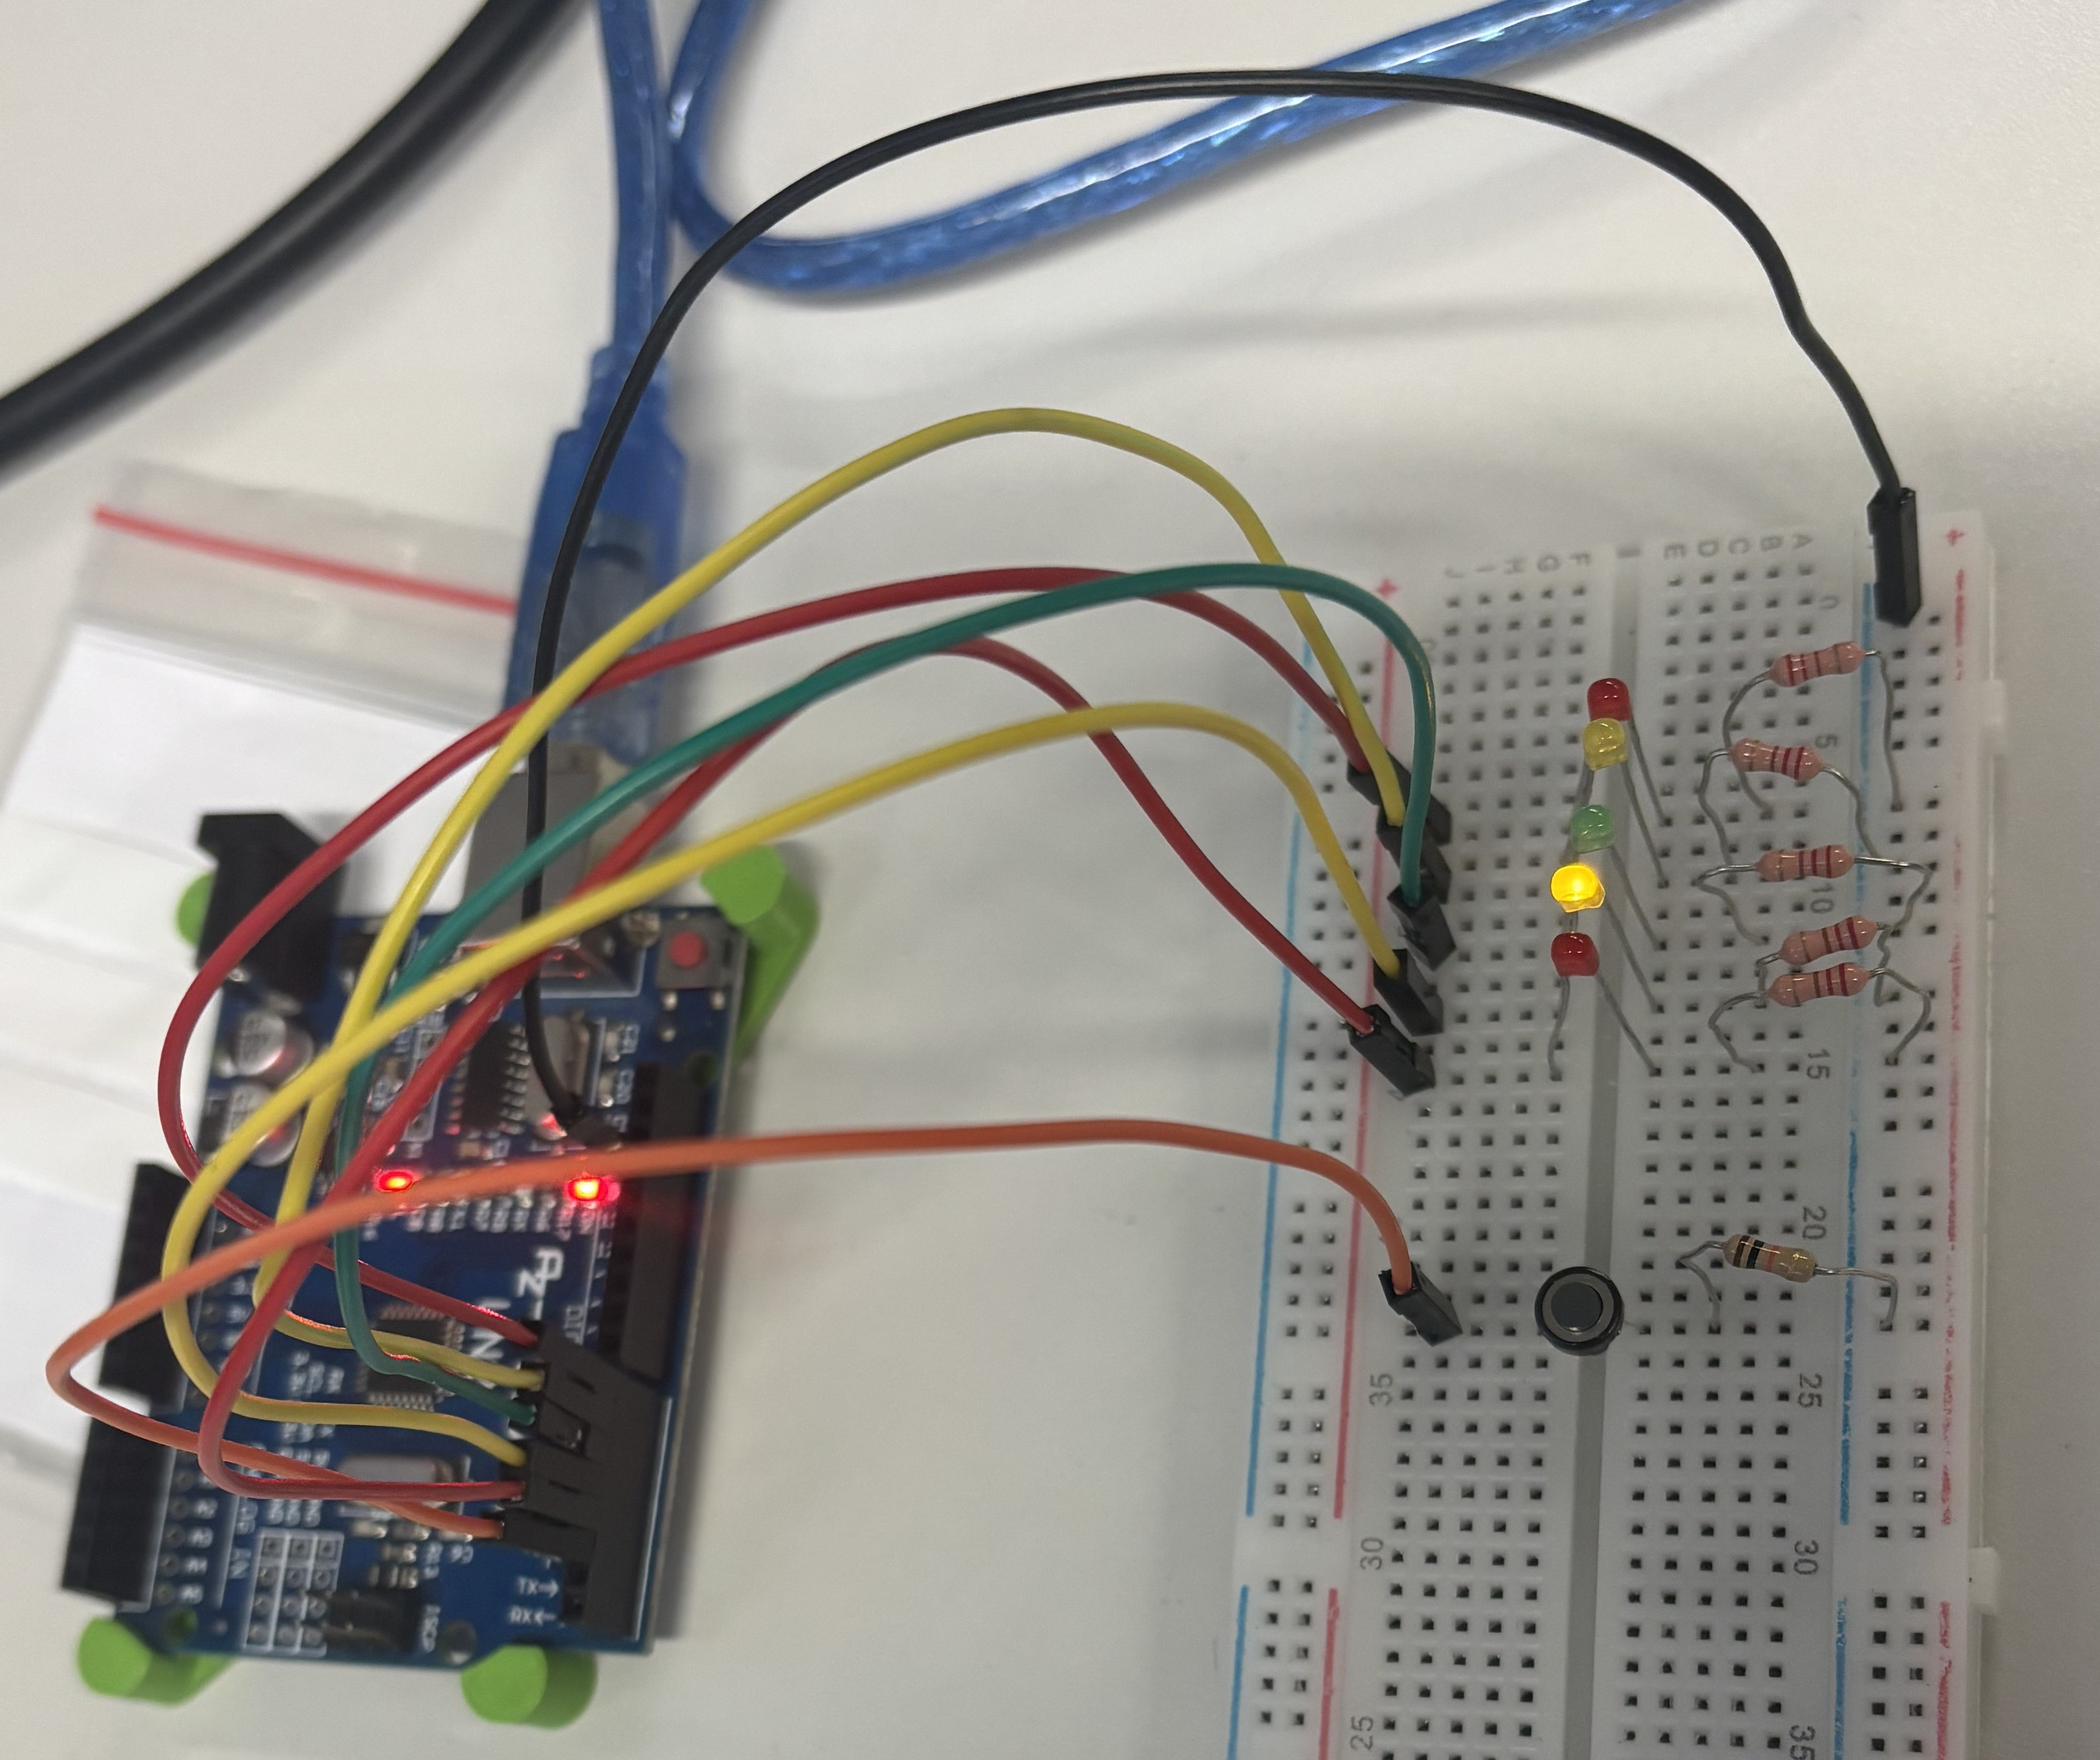
\includegraphics[height=5cm]{latex/images/fotos/2.JPEG}
    \caption{Verdrahtung am Steckbrett.}
\end{figure}

\newpage
\subsubsection{Implementierung}

\lstinputlisting[
    lastline=11,
    caption={Globale Variablen und Definitionen}
]{../02-Reaktionsspiel/react/react.ino}

\lstinputlisting[
    firstline=13,
    caption={Setup und Loop}
]{../02-Reaktionsspiel/react/react.ino}

\subsection{Ergebnisse}
Bei jedem drücken des Tasters während die grüne LED leuchtete wurde das Spiel beschleunigt. Bei falschem drücken wurde das Spiel von neu gestartet. 